\section{Discussion}\label{sec:discussion}
\subsection{Repulsive force from walls}
In chapter 3 we have seen the formulas for calculating the repulsive forces from the wall and other agents are very similar, both are exponential functions decreasing with some distance, which makes us wonder if both come from the same origin.\\

\begin{itemize}
\item The difference between those two repulsive forces is basically one is from a single point and the other is from an object that has a dimension much larger than a single agent. If we imagine our agents are particles with negative charge, then there is a pair of repulsive forces which has direction along the line connecting the two particles and magnitude depending on the distance between them. Further we can put lots of particles along a bar, see Figure
Summing up all the repulsive forces from each particle on the bar will give the repulsive force that the charged bar on the single particle $\alpha$.

\item Applying the idea above to analyse our wall repulsion, as a simple start we place the agent $\alpha$ a distance $ d $ away from the wall which as a length $L$, and by symmetry we know the resulting force must point vertically downwards, see Figure.\\

Integrating the forces can be written as:

\begin{equation}\label{integ}
\vec{f_{\alpha B}} = 
\int_0^L \! \vec{f_{\alpha\beta}} \, \mathrm{d}l
\end{equation}

\item When the repulsive force is known, the expression for the wall potential can be calculated, which can be done by integrating the force along a path. Normally the potential at some position is defined as the work done on the particle by that potential field when the particle is moved from that position to infinitely far away.

\begin{equation}\label{pot}
	U_{B}= \int_{\vec{r_{\alpha}}�}^{text{f}\infty} \! \vec{f_{\alpha B}} \cdot \, \text{d}\vec{r_{\alpha}} 
\end{equation}

\item In some article [Helbing 2000], the repulsive force from the wall is given by:
\begin{equation}\label{helbing2000}
\vec{f_{\alpha B}} = 
	\left( 
			\left[ 
	A exp 
				\left[ 
						\left(  
							r_{\alpha}-d_{\alpha B}
						\right)  / B
				\right] +kg 
					\left( 
						r_{\alpha}-d_{\alpha B} 
					\right) 
			\right] 
		\right)
	\vec{n_{B}^{\alpha}}-\kappa g 
	\left(
		r_{\alpha}-d_{\alpha B}
	\right) 
	\left(
			\vec{V_{\alpha}}\cdot \vec{t_{iw}}
	\right) 
\vec{t_{iw}}
\end{equation}

where $ r_{\alpha} $,  $ \vec{V_{\alpha}} $ are the radius and velocity of agent $ \alpha $ as we noted before, $ A $, $ B $, $ k $, $ \kappa $ are constants, $ d_{\alpha B} $ is the distance from the agent to the wall, $ \vec{n_{B}^{\alpha}} $ is a normal vector from the wall, $ \vec{t_{iw}} $ is a tangent vector to the wall. $ g $ is a function of some variable.\\
In this expression, the wall repulsion force to agent $ \alpha $ is not always perpendicular to the wall, but the force has two components, one perpendicular to the wall and the other tangent to the wall. Particularly the tangent component depends on the velocity of $ \alpha $. However, in Helbing's latest articles he does not show the expression of Equation \ref{helbing2000}, but use the gradient of potential instead. 
\end{itemize}

\subsubsection{Discussion on walls in special cases.}
In the general case of the repulsive force on a pedestrian, $\alpha$, from a wall nearby is given as a function of the vector from the nearest point. This point we calculate by finding the point that makes the vector form $\alpha$ to the wall be perpendicular to to vector that is the wall. In some cases though the point won't be on the wall it self. This of course makes no sense since you would then be repulsed by a non existing part of the wall meaning that you would avoid free areas which makes no sense. In this case you would have to use the end point of the wall. But doing this can make some unrealistic behavior as well, if the walls have the right composition. 

Let's start out by looking at a case with no problem. A case with no problems is a room where the angles between the walls is less than $180^o$, i.e. a squared room where they are $90^o$. For a pedestrian close to the corner between two walls, you would calculate the repulsive force from both of the walls. This you do in order for the pedestrian to avoid going through either one of the walls. When you do this you get a force directly away from each of the walls. This clearly makes sense and there is no problem in doing so.

\begin{figure}
\centering
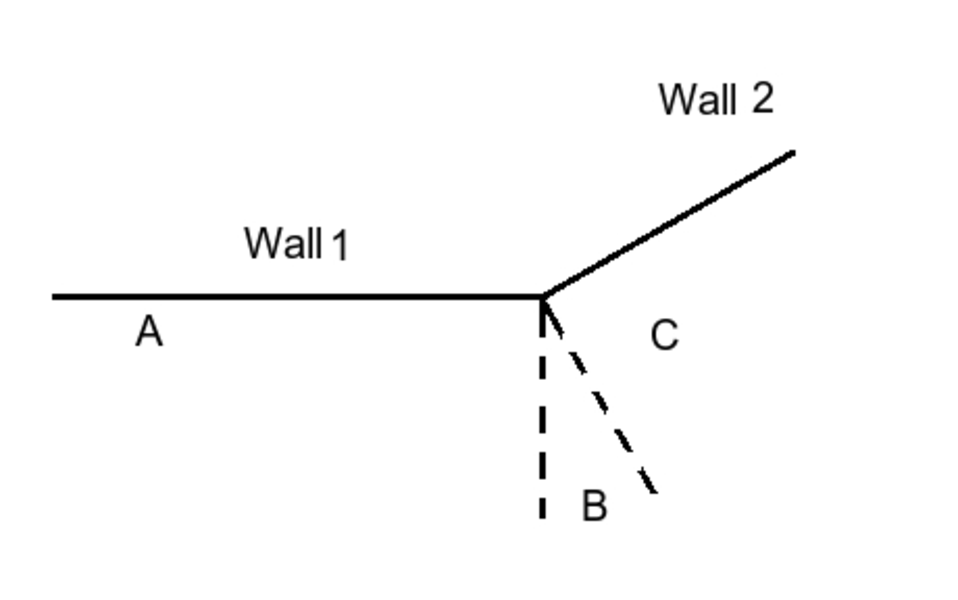
\includegraphics[scale=0.5]{figures/Thewall.pdf}
\caption{Her you can se two walls joint together. In the area `A` a pedestrian will only be perpendicular the first wall. In `B` there is no points perpendicular to any of the walls. And in `C` it is only the second wall that har points perpendicular to the pedestrians.  }
\label{fig:wallcase}
\end{figure}

This case were the angle between two walls is greater than $180^o$ could on the other hand give some problems if not handeled correctly. The case is sketched in figure \ref{fig:wallcase}. Here the are 3 different areas that a pedestrian $\alpha$ can be in. The area A where $\alpha$ is only perpendicular to wall $1$, in area B, $\alpha$ will not be perpendicular to any of the walls and in C he will be only perpendicular to wall 2. If a pedestrian is in area B then we would calculate the forces from the end point of the walls. This will be from the point where the two walls meet together. This will give you a double repulsion from one point and that doesn't make sense. Also when you are in are A or C you would get a repulsive force from a second wall you would be of no risk of going into and in many situations couldn't see because the first wall is blocking the sight. This of course doesn't make any sense too. So the way that we handle this situation is the following. When the angle between the walls is greater than $180^o$, from a pedestrian $\alpha$ point of view, you should look at the two walls as one, in the way that you will only calculate one force from the walls. In area A or C only the closest point on the closest wall should affect you. In the case of $\alpha$ being in area B the walls themselves   doesn't matter, only the vector going from the conjoint point of the walls to $\alpha$, should affect and only one time. Doing this, there should be no unrealistic scenarios.


\subsection{The repulsive force between agents in $ \Re ^{3}$}
From the given formula for calculating the repulsive force between agents in the description of the model, the part calculating the force to keep the personal space can be omitted when the agents are rather close to each other, then the calculation can be reduced as Equation (\ref{eq:re}).

\begin{equation}\label{eq:re}
\overrightarrow{f_{\alpha\beta}}(t) = A_{\alpha}^{2} exp\left[ \frac{r_{\alpha\beta} - d_{\alpha}\beta}{B_{\alpha}^{2}}\right]  \overrightarrow{n_{\alpha\beta}}
\end{equation}

Taking the norms of both sides of Equation (\ref{eq:re}), we can draw the relation between the value of 
$\overrightarrow{f_{\alpha\beta}}(t)$ and $d_{\alpha \beta}$, as in Figure (\ref{fig:physicalinteraction})
\\
\begin{figure}
\centering
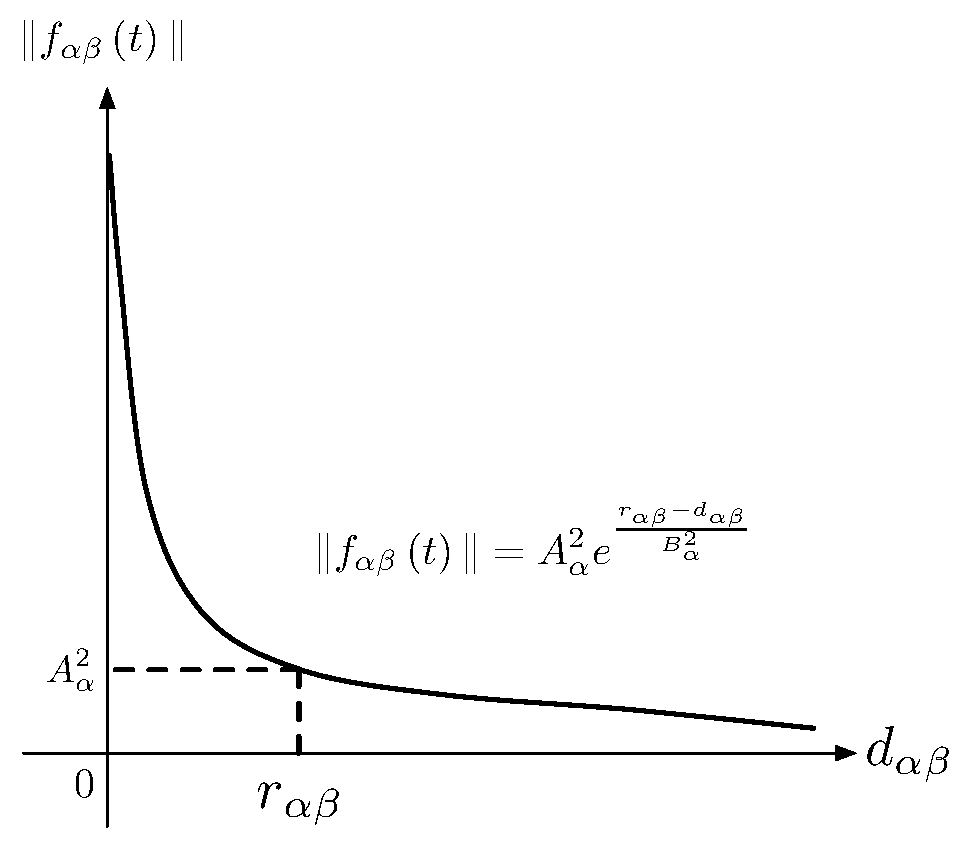
\includegraphics[scale=0.45]{Figures/physicalinteraction.pdf} 
\caption{The function about the interaction force $\vec{f_{\alpha\beta}}(t)$ and the distance between two agents
$d_{\alpha\beta}$ }\label{fig:physicalinteraction}
\end{figure}

There is one intersection of the graph and the axis $ \left( 0, A_{\alpha}^{2} exp\left( \frac{r_{\alpha\beta} }{B_{\alpha}^{2}}\right)  \right)  $. If put into the constants, we will be able to get a maximum value of $ f_{\alpha\beta}(t) $, since the distance between agents cannot be negative. Here we set $ A_{\alpha}^{2} = 3 m/s^{2} $, $ r_{\alpha\beta} = 0.6 m $, and $ B_{\alpha}^{2} = 0.2 m $, so $ f_{\alpha\beta}(t)^{max} \doteq 60 m/s^{2} $, which is about six times the gravitational acceleration and represents a rather large force between agents (as large as six person's weight). \\\\
However, we notice that the effective part of the force calculated above is only the horizontal 
component that enables the agent to move horizontally in the plane where we do the simulation, 
but the reality is that the agents sometimes are also able to move vertically, for example, 
by stepping upon other people when they cannot take the pushing force from the surrounding agents. 
When that happens, the horizontal component of the repulsive force becomes smaller even if 
$d_{\alpha\beta}$ is kept the same.	
Therefore, a qualitative modification of dependence between $ f_{\alpha\beta}(t) $ and $ d_{\alpha\beta} $ could be:
\begin{figure}[hb]   
\centering
    {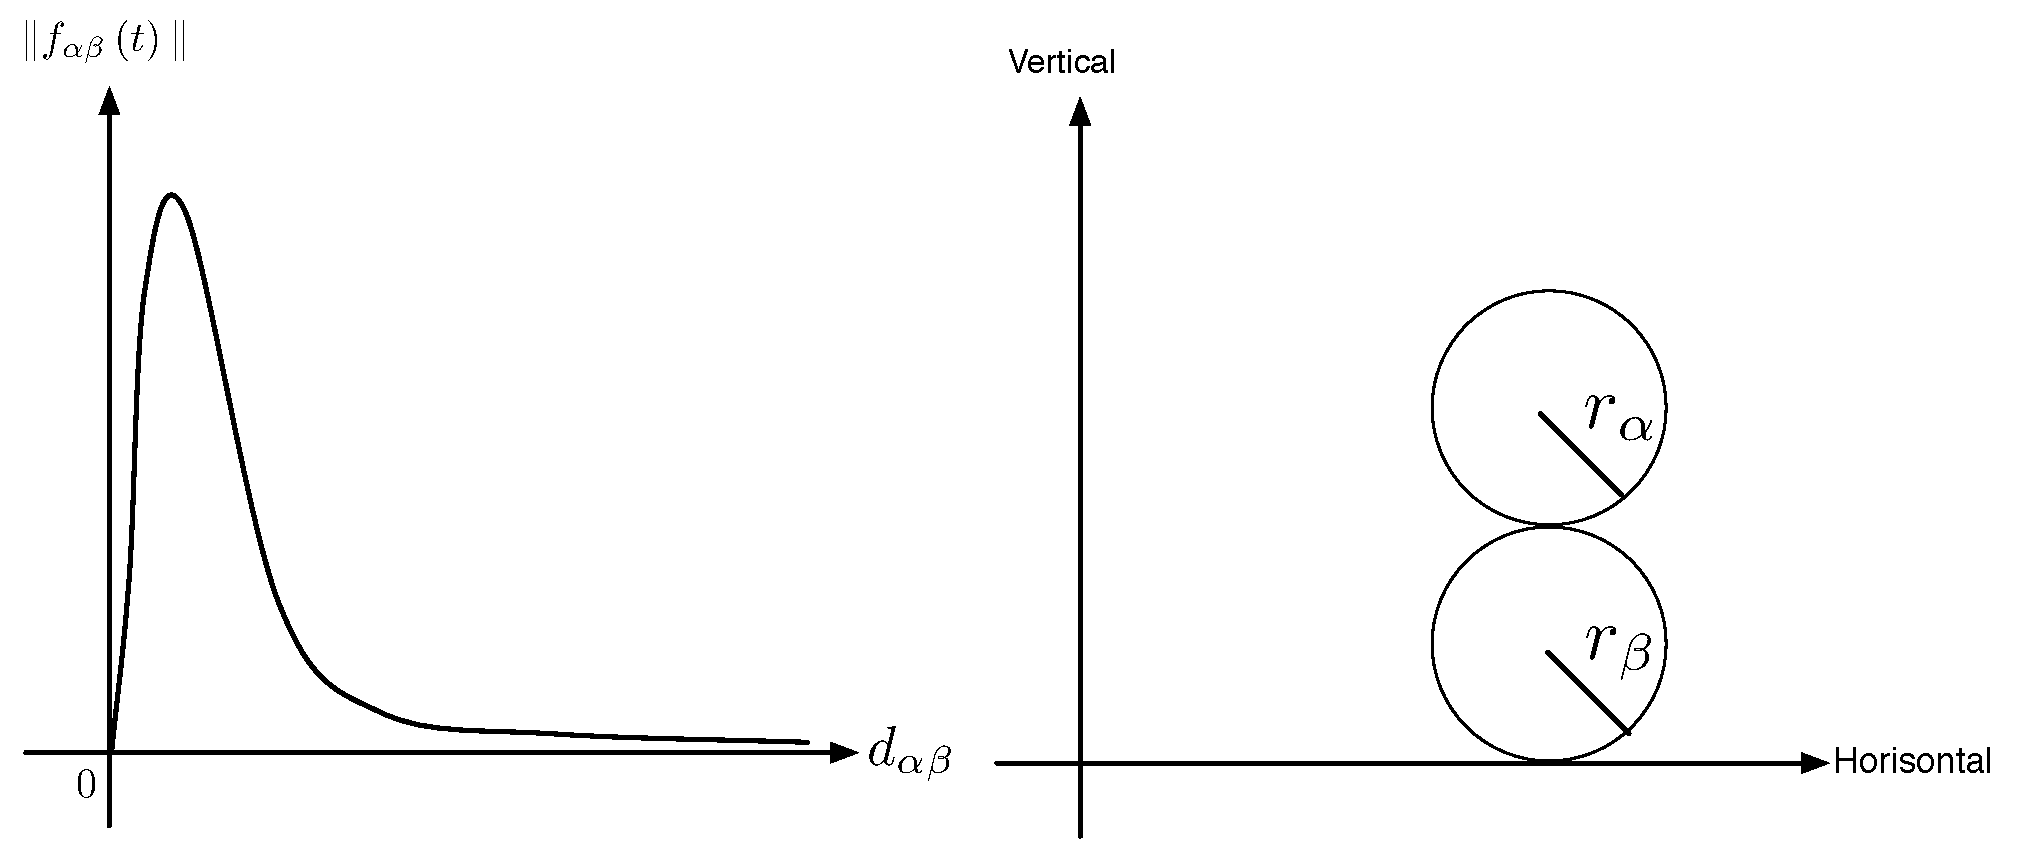
\includegraphics[scale=0.35]{Figures/ForceOverlapping.pdf}} 
    \caption{}
    \label{forceoverlapping}
\end{figure}
\\
\subsection{Use social force in further calculation}
use the value of forces to predict, as they are partly not real forces, the measurement does not reflect the reality in some range.
Pressure